%%%%%%%%%%%%%%%%%%%%%%%%%%%%%%%%%%%%%%%%%%%%%%%%%%%%%%%%%%%%%%%%%%%%%%%%%%%%%%%%%%%%%%%%%%
% Ceci est le fichier principal du template template à utiliser pour les rapports du     %
% projet 1 (Construction de Programme) d'INFO0947.                                       %
%                                                                                        %
% Vous devez décommenter et compléter les commandes introduites plus bas (intitule, ...) %
% avant de pouvoir compiler le fichier LaTeX.  Pensez à configurer votre Makefile en     %
% conséquence.                                                                           %
%                                                                                        %
% Le contenu et la structure du rapport sont imposés.  Vous devez compléter les          %
% différents fichiers .tex inclus dans ce fichier avec votre production.                 %
%%%%%%%%%%%%%%%%%%%%%%%%%%%%%%%%%%%%%%%%%%%%%%%%%%%%%%%%%%%%%%%%%%%%%%%%%%%%%%%%%%%%%%%%%%

% !TEX root = ./main.tex
% !TEX engine = latexmk -pdf
% !TEX buildOnSave = true
\documentclass[a4paper, 11pt, oneside]{article}

\usepackage[utf8]{inputenc}
\usepackage[T1]{fontenc}
\usepackage[french]{babel}
\usepackage{array}
\usepackage{shortvrb}
\usepackage{listings}
\usepackage[fleqn]{amsmath}
\usepackage{amsfonts}
\usepackage{fullpage}
\usepackage{enumerate}
\usepackage{graphicx}             % import, scale, and rotate graphics
\usepackage{subfigure}            % group figures
\usepackage{alltt}
\usepackage{url}
\usepackage{indentfirst}
\usepackage{eurosym}
\usepackage{listings}
\usepackage{color}
\usepackage[table,xcdraw,dvipsnames]{xcolor}

% Change le nom par défaut des listing
\renewcommand{\lstlistingname}{Extrait de Code}


\definecolor{mygray}{rgb}{0.5,0.5,0.5}
\newcommand{\coms}[1]{\textcolor{MidnightBlue}{#1}}

\lstset{
    language=C, % Utilisation du langage C
    commentstyle={\color{MidnightBlue}}, % Couleur des commentaires
    frame=single, % Entoure le code d'un joli cadre
    rulecolor=\color{black}, % Couleur de la ligne qui forme le cadre
    stringstyle=\color{RawSienna}, % Couleur des chaines de caractères
    numbers=left, % Ajoute une numérotation des lignes à gauche
    numbersep=5pt, % Distance entre les numérots de lignes et le code
    numberstyle=\tiny\color{mygray}, % Couleur des numéros de lignes
    basicstyle=\tt\footnotesize,
    tabsize=3, % Largeur des tabulations par défaut
    keywordstyle=\tt\bf\footnotesize\color{Sepia}, % Style des mots-clés
    extendedchars=true,
    captionpos=b, % sets the caption-position to bottom
    texcl=true, % Commentaires sur une ligne interprétés en Latex
    showstringspaces=false, % Ne montre pas les espace dans les chaines de caractères
    escapeinside={(>}{<)}, % Permet de mettre du latex entre des <( et )>.
    inputencoding=utf8,
    literate=
  {á}{{\'a}}1 {é}{{\'e}}1 {í}{{\'i}}1 {ó}{{\'o}}1 {ú}{{\'u}}1
  {Á}{{\'A}}1 {É}{{\'E}}1 {Í}{{\'I}}1 {Ó}{{\'O}}1 {Ú}{{\'U}}1
  {à}{{\`a}}1 {è}{{\`e}}1 {ì}{{\`i}}1 {ò}{{\`o}}1 {ù}{{\`u}}1
  {À}{{\`A}}1 {È}{{\`E}}1 {Ì}{{\`I}}1 {Ò}{{\`O}}1 {Ù}{{\`U}}1
  {ä}{{\"a}}1 {ë}{{\"e}}1 {ï}{{\"i}}1 {ö}{{\"o}}1 {ü}{{\"u}}1
  {Ä}{{\"A}}1 {Ë}{{\"E}}1 {Ï}{{\"I}}1 {Ö}{{\"O}}1 {Ü}{{\"U}}1
  {â}{{\^a}}1 {ê}{{\^e}}1 {î}{{\^i}}1 {ô}{{\^o}}1 {û}{{\^u}}1
  {Â}{{\^A}}1 {Ê}{{\^E}}1 {Î}{{\^I}}1 {Ô}{{\^O}}1 {Û}{{\^U}}1
  {œ}{{\oe}}1 {Œ}{{\OE}}1 {æ}{{\ae}}1 {Æ}{{\AE}}1 {ß}{{\ss}}1
  {ű}{{\H{u}}}1 {Ű}{{\H{U}}}1 {ő}{{\H{o}}}1 {Ő}{{\H{O}}}1
  {ç}{{\c c}}1 {Ç}{{\c C}}1 {ø}{{\o}}1 {å}{{\r a}}1 {Å}{{\r A}}1
  {€}{{\euro}}1 {£}{{\pounds}}1 {«}{{\guillemotleft}}1
  {»}{{\guillemotright}}1 {ñ}{{\~n}}1 {Ñ}{{\~N}}1 {¿}{{?`}}1
}
\newcommand{\tablemat}{~}

%%%%%%%%%%%%%%%%% TITRE %%%%%%%%%%%%%%%%
% Complétez et décommentez les définitions de macros suivantes :
\newcommand{\intitule}{Construction de programme}
\newcommand{\GrNbr}{27}
\newcommand{\PrenomUN}{Alexandru}
\newcommand{\NomUN}{Dobre}
\newcommand{\PrenomDEUX}{Sami}
\newcommand{\NomDEUX}{Ouazouz}

\renewcommand{\tablemat}{\tableofcontents}

%%%%%%%% ZONE PROTÉGÉE : MODIFIEZ UNE DES DIX PROCHAINES %%%%%%%%
%%%%%%%%            LIGNES POUR PERDRE 2 PTS.            %%%%%%%%
\title{INFO0947: \intitule}
\author{Groupe \GrNbr : \PrenomUN~\textsc{\NomUN}, \PrenomDEUX~\textsc{\NomDEUX}}
\date{}
\begin{document}

\maketitle
\newpage
\tablemat
\newpage

%%%%%%%%%%%%%%%% RAPPORT %%%%%%%%%%%%%%%

% Inclusion des différentes sections

\section{Introduction}\label{introduction}

Ce projet consistait à développer une implémentation du jeu "Five or More", 
où le joueur doit déplacer des boules de différentes couleurs sur une grille en créant des 
alignements d'au moins cinq boules de même couleur, générant ainsi du score. 
Notre travail a porté sur la conception d'une interface graphique 
utilisant la bibliothèque GTK2+, ainsi que sur l'implémentation de la logique 
de jeu en langage C avec divers algorithmes.

% !TEX root = ./main.tex
%%%%%%%%%%%%%%%%%%%%%%%%%%%%%%%%%%%%%%%%%%%%%%%%%%%%%%%%%%%%%%%%%%%%%%%%%%%%%%%%%%%%%%%%%%
% Dans cette section, introduisez toutes les notations mathématiques que vous jugez      %
% utiles à la réalisation du projet.                                                     %
%%%%%%%%%%%%%%%%%%%%%%%%%%%%%%%%%%%%%%%%%%%%%%%%%%%%%%%%%%%%%%%%%%%%%%%%%%%%%%%%%%%%%%%%%%
\section{Formalisation du Problème}\label{formalisation}
%%%%%%%%%%%%%%%%%%%%%%%%%%%%%%%%%%%

Soit \textbf{prefixe\_suffixe(*T, N)} , une notation telle que:
\begin{itemize}
   \item $T$ un tableau d'entiers.
   \item $N$ est la taille du tableau $(N \geq 0)$.
\end{itemize}

\vspace{0.2cm}
On a $prefixe\_suffixe (*T, N) \equiv \forall k, 0 \leq k \leq N-1 : T[0, k] = T[N-k, N-1]$.

\vspace{0.4cm}
Soit \textbf{est\_pref\_suff(T, k, N)} une notation telle que:
\begin{itemize}
   \item $T$ est un tableau d'entiers
   \item $k$ est la taille du préfixe/suffixe à tester
   \item $N$ est la taille du tableau
\end{itemize}

\vspace{0.2cm}
$est\_pref\_suff(T, k, N) \equiv \forall i, 0 \leq i < k : T[i] = T[N-k+i]$

\vspace{0.4cm}
Soit \textbf{max\_prefixe\_suffixe(*T, i , N)} une notation pour le plus long 
préfixe-suffixe de T telle que:
\begin{itemize}
   \item $T$ est un tableau d'entiers
   \item $i$ est la position de comparaison
   \item $N$ est la taille du tableau
\end{itemize}

\vspace{0.2cm}
$max\_prefixe\_suffixe(*T, i , N) \equiv max\{k | 0 \leq k < N \wedge est\_pref\_suff(T, K, N)\}$


% !TEX root = ./main.tex
%%%%%%%%%%%%%%%%%%%%%%%%%%%%%%%%%%%%%%%%%%%%%%%%%%%%%%%%%%%%%%%%%%%%%%%%%%%%%%%%%%%%%%%%%%
% Dans ce fichier, vous devez définir (Input/Output/O.U.) proprement et clairement le    %
% problème.
%
% Il est aussi demandé de réaliser une analyse complète (i.e., découpe en SPs)           %
%%%%%%%%%%%%%%%%%%%%%%%%%%%%%%%%%%%%%%%%%%%%%%%%%%%%%%%%%%%%%%%%%%%%%%%%%%%%%%%%%%%%%%%%%%

\section{Définition et Analyse du Problème}\label{analyse}
%%%%%%%%%%%%%%%%%%%%%%%%%%%%%%%%%%%%%%%%%%%%


% !TEX root = ./main.tex
%%%%%%%%%%%%%%%%%%%%%%%%%%%%%%%%%%%%%%%%%%%%%%%%%%%%%%%%%%%%%%%%%%%%%%%%%%%%%%%%%%%%%%%%%%
% Dans cette section, spécifiez formellement chacun des sous-problèmes.                  %
%%%%%%%%%%%%%%%%%%%%%%%%%%%%%%%%%%%%%%%%%%%%%%%%%%%%%%%%%%%%%%%%%%%%%%%%%%%%%%%%%%%%%%%%%%
\section{Specifications}\label{specifications}
%%%%%%%%%%%%%%%%%%%%%%%%

%  \item \textbf{SP1} : \'Enumération des tailles possbiles de préfixe-suffixe.
%\item \textbf{SP2} : Comparer les valeurs de préfixe et de suffixe.

\subsection{Sous-problème 1}
Nous voulons écrire une boucle dans laquelle $k$ balaye toutes les valeurs
possibles pour le préfixe-suffixe. Pour ceci définissons la fonction:
\begin{itemize}
   \item \textbf{Input:}
      \begin{itemize}
         \item $N$, la taille du tableau
      \end{itemize}
   \item \textbf{Output:}
      \begin{itemize}
         \item $k$, la taille du préfixe-suffixe
      \end{itemize}
   \item \textbf{Caractérisation de l'input:}
      \begin{itemize}
         \item $N$ est un entier non signé tel que $N \geq 0$
         \item \textbf{unsigned int} N
      \end{itemize}
\end{itemize}

\vspace{0.4cm}
Il nous faut donc écrire une boucle while qui va balayer toutes les valeurs 
possibles de $k$ de $N-1$ à 0.
\begin{itemize}
   \item \textbf{Déclaration du compteur:}
      \begin{itemize}
         \item \textbf{unsigned int} $k = N-1$
      \end{itemize}
   \item \textbf{Nombres de tours dans la boucle:}
      \begin{itemize}
         \item $N-1$
      \end{itemize}
   \item \textbf{Gardien de boucle:}
      \begin{itemize}
         \item $k > 0$
      \end{itemize}
   \item \textbf{Corps de Boucle:}
   \begin{itemize}
      \item \textbf{Comparer les valeurs de préfixe et de suffixe:}
      \begin{itemize}
         \item SP2
      \end{itemize}
      \item Décrémenter k
   \end{itemize}
\end{itemize}

\begin{lstlisting}[language=C, caption=SP1]
unsigned int k = N - 1;
while (k > 0) {
   // SP2
   k--;
}
\end{lstlisting}

\subsection{Sous-problème 2}
Nous voulons écrire une boucle dans laquelle on compare les valeurs de préfixe
et de suffixe. Pour ceci définissons la fonction:
\begin{itemize}
   \item \textbf{Input:}
      \begin{itemize}
         \item $T$, le tableau d'entiers
         \item $N$, la taille du tableau
         \item $k$, la taille du préfixe-suffixe
         \item $i$, le compteur de la boucle
      \end{itemize}
   \item \textbf{Output:}
      \begin{itemize}
         \item $k$, la taille du préfixe-suffixe
      \end{itemize}
   \item \textbf{Caractérisation des inputs:}
      \begin{itemize}
         \item $N$ est un entier non signé tel que $N \geq 0$
         \item \textbf{unsigned int} $N$
         \item $k$ est un entier non signé tel que $0 \leq k < N$
         \item \textbf{unsigned int} $k = N - 1$
         \item $i$ est un entier non signé tel que $0 \leq i < k$
         \item \textbf{unsigned int} $i = 0$
         \item $T$ est un tableau d'entiers tel que $T[0, N-1]$
         \item \textbf{int} $T[N]$
      \end{itemize}
\end{itemize}
%
%
%
%
%
%%%%%%%%%%%%%%%%%%%%%%%%%%%% A CONTINUER %%%%%%%%%%%%%%%%%%%%%%%%%%%%%%%%

\vspace{0.4cm}
Il nous faut donc écrire une boucle while qui va balayer toutes les valeurs
possibles de $i$ de 0 à k-1 et trouver des correspondances entre les
valeurs de préfixe $i$ et de suffixe $N-k+i$.
\begin{itemize}
   \item \textbf{Déclaration du compteur:}
      \begin{itemize}
         \item \textbf{unsigned int} $i = 0$
      \end{itemize}
   \item \textbf{Nombres de tours dans la boucle:}
      \begin{itemize}
         \item $k$
      \end{itemize}
   \item \textbf{Gardien de boucle:}
   \item \textbf{Condition de sortie:}
      \begin{itemize}
         \item $i < k $\space$ \&\& $\space$ T[i] == T[N - k +i]$
      \end{itemize}
   \item \textbf{Corps de Boucle:}
   \begin{itemize}
      \item \textbf{Vérifier si $i$ et $k$ sont égaux:}
      \begin{itemize}
      \item if (i == k)
      \end{itemize}
      \item Incrémenter i
   \end{itemize}
\end{itemize}

\vspace{0.4cm}
\begin{lstlisting}[language=C, caption=SP2]
unsigned int i = 0;
while(i < k && T[i] == T[N - k +i]){
   i++;
   }
   if (i == k){
      return k;
   }
   else{
      i = 0;
}
\end{lstlisting}

% !TEX root = ./main.tex
%%%%%%%%%%%%%%%%%%%%%%%%%%%%%%%%%%%%%%%%%%%%%%%%%%%%%%%%%%%%%%%%%%%%%%%%%%%%%%%%%%%%%%%%%%
% Dans cette section, indiquez et décrivez tous les Invariants nécessaires.              %
%                                                                                        %
% Pour chaque SP nécessitant un Invariant (une sous-section/SP):                         %
% - Donnez l'Invariant Graphique                                                         %
% - Donnez l'Invariant Formel correspondant à l'Invariant Graphique                      %
% Pensez à utiliser les notations définies précédemment.                                 %
%%%%%%%%%%%%%%%%%%%%%%%%%%%%%%%%%%%%%%%%%%%%%%%%%%%%%%%%%%%%%%%%%%%%%%%%%%%%%%%%%%%%%%%%%%
\section{Invariants}\label{invariants}
%%%%%%%%%%%%%%%%%%%%
\subsection{Explications}
La raison d'être de cette section est de définir les invariants nécessaires à la
construction du programme. Les invariants sont des propriétés qui doivent être
vérifiées à chaque étape de l'exécution du programme. Ils permettent de garantir
que le programme fonctionne correctement et produit les résultats attendus. Il y
a une règle qui est que chaque boucle nécessite un invriant. Nous aurons donc 2
invariants graphiques et 2 invariants formels

Nous allons donc définir les invariants graphiques. Le premier aura pour objectif
de définir la boucle de décrementation de $k$ et le seconde couvrira la boucle
qui compare les valeurs du tableau entre $T[i]$ et $T[N-k+i]$.

\subsection{SP1}
\subsubsection{Invariant Graphique}
Pour le premier invariant, nous allons définir la boucle de décrementation de $k
$. La valeur de $k$ est initialisée à $N - 1$ et elle est décrémentée jusqu'à ce
qu'elle atteigne 0. Attention, elle atteint zéro uniquement si lors du SP2 nous 
n'avons trouvé aucune correspondance dans le tableau.
\begin{figure}[h]
   \centering
   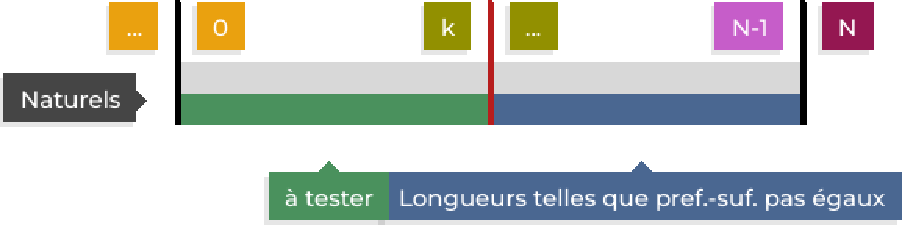
\includegraphics[width=0.5\textwidth]{sp1.pdf}
   \caption{Invariant graphique 1}
   \label{fig:invariant1}
\end{figure}

Le critère d'arrêt de la boucle est $k ==0$. Donc, le gardien de boucle sera
$k > 0$.

\subsubsection{Invariant Formel}

\begin{center}
   \fbox{
      \begin{minipage}{0.5\textwidth}
      \begin{center}
      $N = N_0$ \\
      $\wedge$ \\
      $ 0 \leq k \leq N - 1$ \\
      $\wedge$ \\
      k != max\_prefixe\_suffixe(*T, i ,N) \\
      \end{center}
      \end{minipage}
   }
\end{center}

\subsection{SP2}
\subsubsection{Invariant Graphique}
Pour le second invariant, nous allons définir la boucle de comparaison entre les
valeurs du tableau entre $T[i]$ et $T[N-k+i]$. La valeur de $i$ est initialisée 
à 0 et elle est incrémentée jusqu'à ce qu'elle atteigne $k$.

\begin{figure}[h]
   \centering
   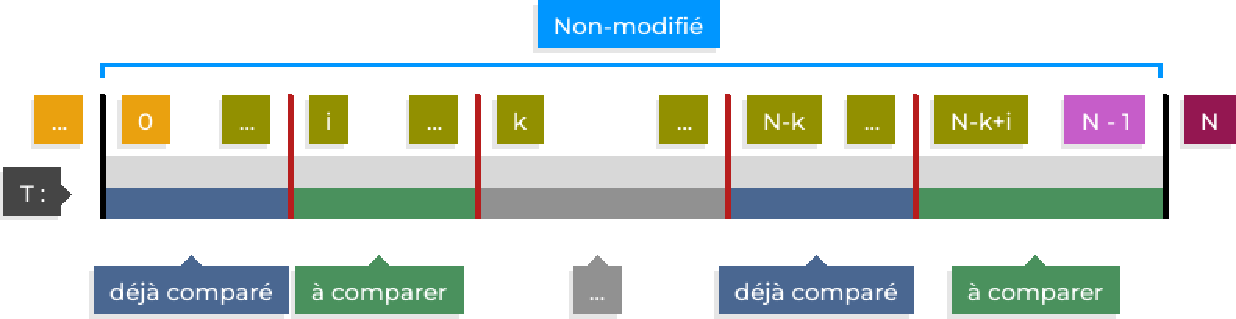
\includegraphics[width=0.5\textwidth]{sp2.pdf}
   \caption{Invariant graphique 2}
   \label{fig:invariant2}
\end{figure}

Le critère d'arrêt de la boucle est $i == k$. Donc, le gardien de boucle sera
$i < k$.
\subsubsection{Invariant Formel}

\begin{center}
   \fbox{
      \begin{minipage}{0.5\textwidth}
      \begin{center}
      $N = N_0 \wedge T = T_0$ \\
      $\wedge$ \\
      $ 0 \leq i < k$ $< N$\\
      $\wedge$ \\
      $\forall i,k, 0 \leq i < k < N$, $est\_pre\_suff$ \\
      \end{center}
      \end{minipage}
   }
\end{center}

% !TEX root = ./main.tex
%%%%%%%%%%%%%%%%%%%%%%%%%%%%%%%%%%%%%%%%%%%%%%%%%%%%%%%%%%%%%%%%%%%%%%%%%%%%%%%%%%%%%%%%%%
% Dans cette section, il est demandé d'appliquer l'approche constructive pour la         %
% construction de votre code.                                                            %
%                                                                                        %
% Pour chaque Sous-Problème (une sous-section/SP):                                       %
% - {Pré} INIT {INV}                                                                     %
% - déterminer le Critère d'Arrêt (et donc le Gardien de Boucle)                         %
% - {INV & B} ITER {INV}                                                                 %
% - {INV & !B} END {Post}                                                                %
% - Fonction de Terminaison (pensez à justifier sur base de l'Invariant Graphique)       %
% (une sous-sous-section/tiret)                                                          %
%%%%%%%%%%%%%%%%%%%%%%%%%%%%%%%%%%%%%%%%%%%%%%%%%%%%%%%%%%%%%%%%%%%%%%%%%%%%%%%%%%%%%%%%%%
\section{Approche Constructive}
%%%%%%%%%%%%%%%%%%%%%%%%%%%%%%%%

\subsection{Sous-problème 1}

Voici les instructions ainsi que la construction instruction par instruction pour le sous-problème 1.
\begin{lstlisting}[caption={Sous-problème 1}]
    (>\coms{\{Pré $\equiv N = N_{0} \land 0 \leq N$\}}<)
    int k = N - 1;
    (>\coms{\{Inv $\equiv N = N_{0} \land 0 \leq N \land k = N - 1 \land k \ne \text{est\_pref\_suff}(\text{*}T, i, N)$\}}<)
    while (k > 0) {
      (>\coms{\{Inv $\land B \equiv N = N_{0} \land 0 \leq N \land k \leq N - 1 \land k \ne \text{est\_pref\_suff}(\text{*}T, i, N) \land k > 0$\}}<)

      (>\coms{\{$N = N_{0} \land 0 \leq N \land 0 < k \leq N - 1 \land k \ne \text{est\_pref\_suff}(\text{*}T, i, N)$\}}<)
      // SP2
      if (i == k){
        (>\coms{\{$N = N_{0} \land 0 \leq N \land 0 < k \leq N - 1 \land k = \text{est\_pref\_suff}(\text{*}T, i, N)$\}}<)
        return k;
      }
      else{
        i = 0;
      }
      k --;
      (>\coms{\{Inv $\land B \equiv N = N_{0} \land 0 \leq N \land k \leq N - 1 \land k \ne \text{est\_pref\_suff}(\text{*}T, i, N)$\}}<)
    }
    (>\coms{\{Inv $\land \lnot B \equiv T = T_{0} \land N \geq 0 \land k = 0$\}}<)
\end{lstlisting}


\subsection{Sous-problème 2}

Voici les instructions ainsi que la construction instruction par instruction pour le sous-problème 2.
\begin{lstlisting}[caption={Sous-problème 2}]
    (>\coms{\{Pré $\equiv N = N_{0} \land T = T_{0} \land 0 < k \leq N - 1$\}}<)
    int i = 0;
    (>\coms{\{Inv $\equiv N = N_{0} \land T = T_{0} \land i = 0 < k \leq N - 1$\}}<)
    while(i < k && T[i] == T[N - k + i]){
      (>\coms{\{Inv $\land B \equiv N = N_{0} \land T = T_{0} \land 0 \leq i < k < N - 1 \land T[i] = T[N - k + i]$\}}<) 
      i++;
      (>\coms{\{$N = N_{0} \land T = T_{0} \land 0 < i \leq k < N - 1 \land T[i] = T[N - k + i]$\}}<)
    }
    (>\coms{\{Inv $\land \lnot B \equiv T = T_{0} \land i == k \lor T[i] \ne T[N - k + i] \land i = \text{max\_pref\_suff}(*T, i, N)$\}}<)
\end{lstlisting}



% !TEX root = ./main.tex
%%%%%%%%%%%%%%%%%%%%%%%%%%%%%%%%%%%%%%%%%%%%%%%%%%%%%%%%%%%%%%%%%%%%%%%%%%%%%%%%%%%%%%%%%%
% Dans cette section, indiquez le code complet (sans assertions intermédiaires) de votre %
% solution                                                                               %
%%%%%%%%%%%%%%%%%%%%%%%%%%%%%%%%%%%%%%%%%%%%%%%%%%%%%%%%%%%%%%%%%%%%%%%%%%%%%%%%%%%%%%%%%%
\section{Code Complet}\label{code}
%%%%%%%%%%%%%%%%%%%%%%%

\subsection{Code du module}
\begin{lstlisting}[caption={prefixe\_suffixe.c}]
    #include <assert.h>
    #include <stdlib.h>
    
    #include "prefixe_suffixe.h"
    
    
    int prefixe_suffixe(int *T, const unsigned N){
      int k = N-1;
      int i = 0;
    
      while (k > 0){
        while (i < k && T[i] == T[N - k +i]) {
          i++;
        } // fin while
        if (i == k) {
          return k;
        }
        else{
          i = 0;
        }
        k--;
      } // fin while
      return 0;
    } // fin prefixe\_suffixe
\end{lstlisting}

\subsection{Code du programme principal}
\begin{lstlisting}[caption={main-prefixe\_suffixe.c}]
    #include <stdio.h>

    #include "prefixe_suffixe.h"
    
    #define N1 9
    #define N2 10
    #define N3 9
    
    int main(){
    
      int T1[N1] = {1,4,2,4,5,1,4,2,4};
      int T2[N2] = {1,2,3,2,1,1,2,3,2,1};
      int T3[N3] = {3,2,3,2,1,2,3,2,1};
      int T4[N1] = {1,1,1,1,1,1,1,1,1};
    
      printf("Longueur plus long préfixe/suffixe de T1: %u\n", 
            prefixe_suffixe(T1, N1));
      printf("Longueur plus long préfixe/suffixe de T2: %u\n", 
            prefixe_suffixe(T2, N2));
      printf("Longueur plus long préfixe/suffixe de T3: %u\n", 
            prefixe_suffixe(T3, N3));
      printf("Longueur plus long préfixe/suffixe de T4: %u\n", 
            prefixe_suffixe(T4, N1));
    }
\end{lstlisting}




% !TEX root = ./main.tex
%%%%%%%%%%%%%%%%%%%%%%%%%%%%%%%%%%%%%%%%%%%%%%%%%%%%%%%%%%%%%%%%%%%%%%%%%%%%%%%%%%%%%%%%%%
% Dans cette section, vous devez étudier complètement la complexité de votre code.       %
% Soyez le plus formel (i.e., mathématique) possible.                                    %
%%%%%%%%%%%%%%%%%%%%%%%%%%%%%%%%%%%%%%%%%%%%%%%%%%%%%%%%%%%%%%%%%%%%%%%%%%%%%%%%%%%%%%%%%%
\section{Complexité}\label{complexite}
%%%%%%%%%%%%%%%%%%%%


% !TEX root = ./main.tex
%%%%%%%%%%%%%%%%%%%%%%%%%%%%%%%%%%%%%%%%%%%%%%%%%%%%%%%%%%%%%%%%%%%%%%%%%%%%%%%%%%%%%%%%%%
% Rédigez ici la conclusion de votre rapport.                                            %
%%%%%%%%%%%%%%%%%%%%%%%%%%%%%%%%%%%%%%%%%%%%%%%%%%%%%%%%%%%%%%%%%%%%%%%%%%%%%%%%%%%%%%%%%%
\section{Conclusion}\label{conclusion}
%%%%%%%%%%%%%%%%%%%%%
Pour conclure, à travers notre rapport, nous avons établi une approche
constructive pour une fonction calculant le plus long
sous-tableau qui est à la fois préfixe et suffixe d'un tableau donné. 
Nous avons défini le problème, formalisé le problème, analysé, découpé en 
sous-problèmes et avons fait une approche constructive sur la base de nos invariants.

\vspace{0.4cm}
Nous avons également calculé la complexité de notre algorithme, qui est $O(n^2)$.
Notre code peut désormais être utilisé pour résoudre le problème de manière efficace et
fiable.

%%%%%%%%%%%%%%%%%%%% FIN DE LA ZONE PROTÉGÉE %%%%%%%%%%%%%%%%%%%%

\end{document}
